\chapter{Pembuatan Aplikasi pada Oracle Apex Online}

\section{Langkah-Langkah Pembuatan Aplikasi Akademik Sederhana APEX}

\begin{enumerate}

\begin{figure}[!htbp]
\item[1]Hal pertama yang perlu dilakukan adalah masuk dan membuat project pada Microsoft Excel. Project tersebut kita membuat beberapa tabel yang terdiri atas tabel mahasiswa, tabel dosen, tabel kuliah, tabel nilai, dan tabel jadwal.Untuk setiap tabel dibuat pada sheet yang berbeda.

    \begin{center}
    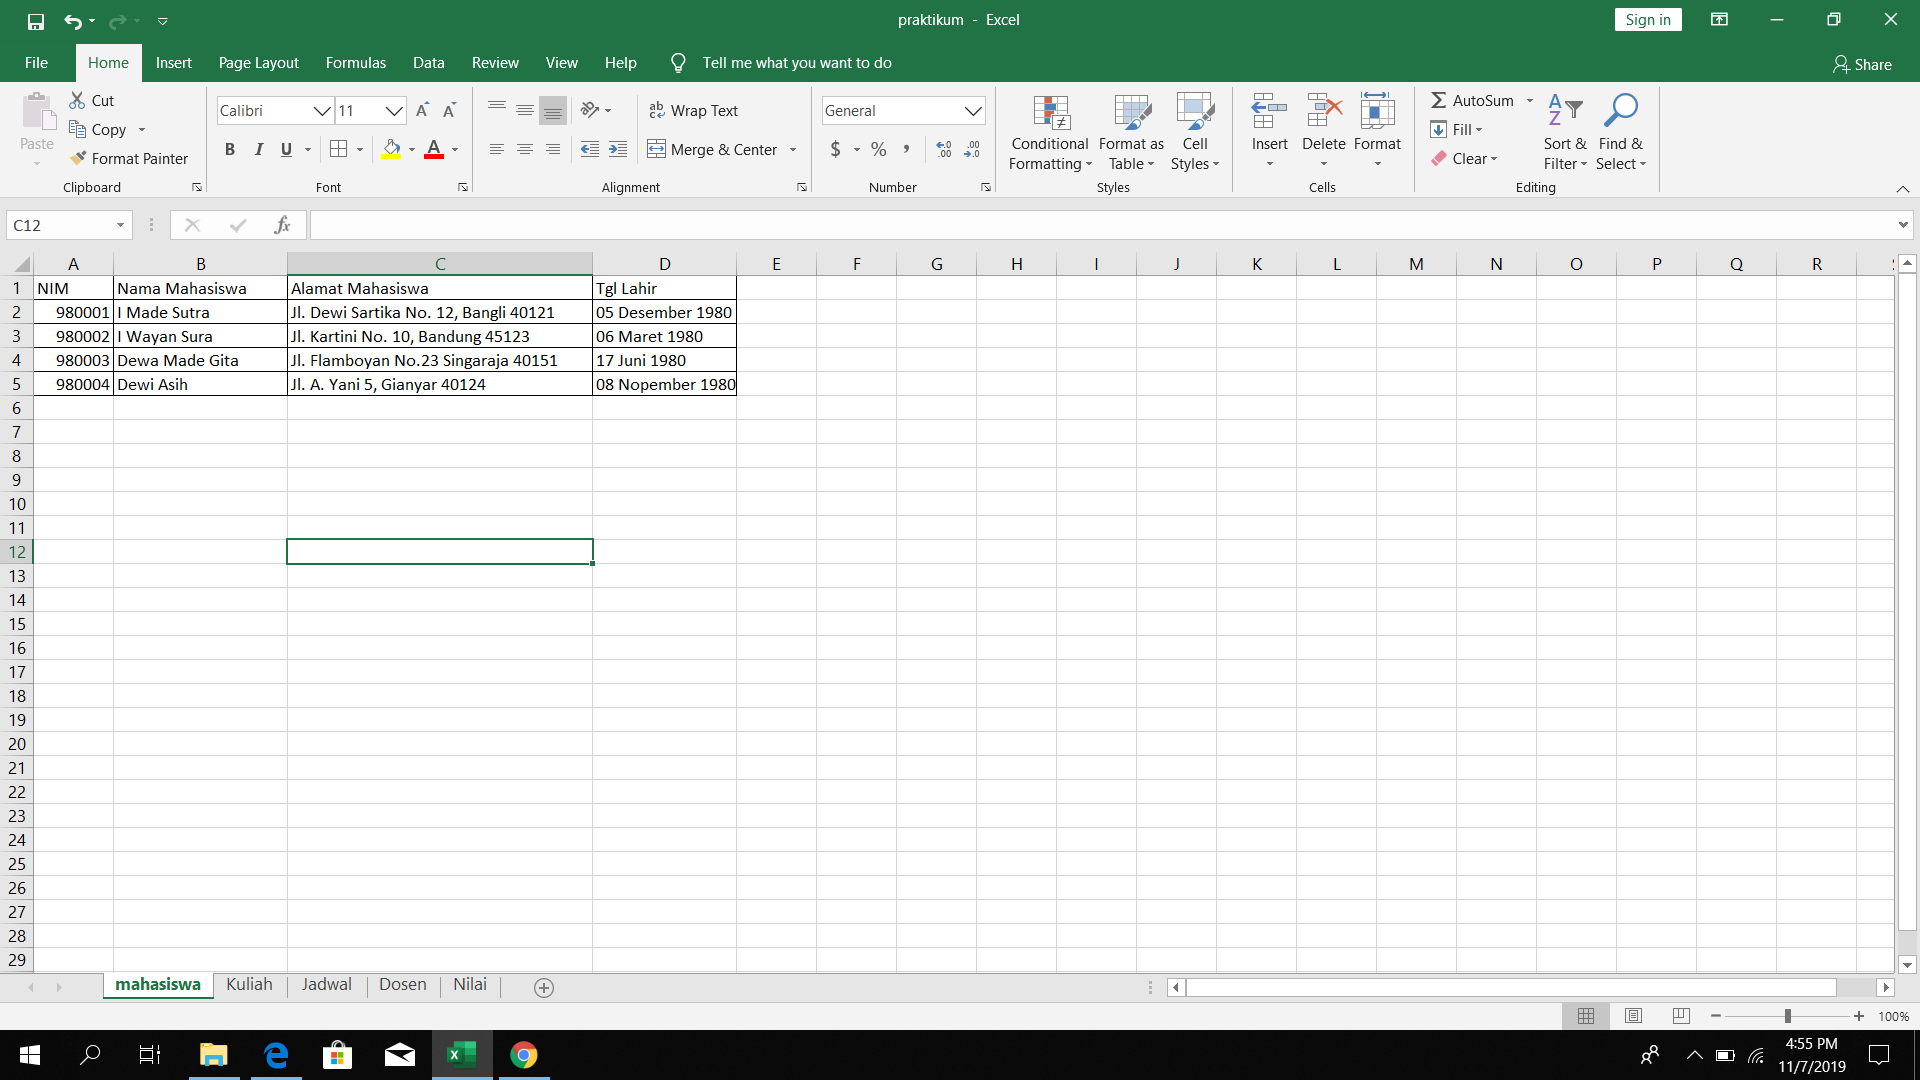
\includegraphics[scale=0.2]{figures/1.png}
    \caption{Membuat tabel pada microsoft excel}
    \end{center}
    \end{figure}

\begin{figure}[!htbp]
\item[2]Setelah membuat 5 tabel pada project di Microsoft Excel, selanjutnya masuk ke aplikasi oracle online.

    \begin{center}
    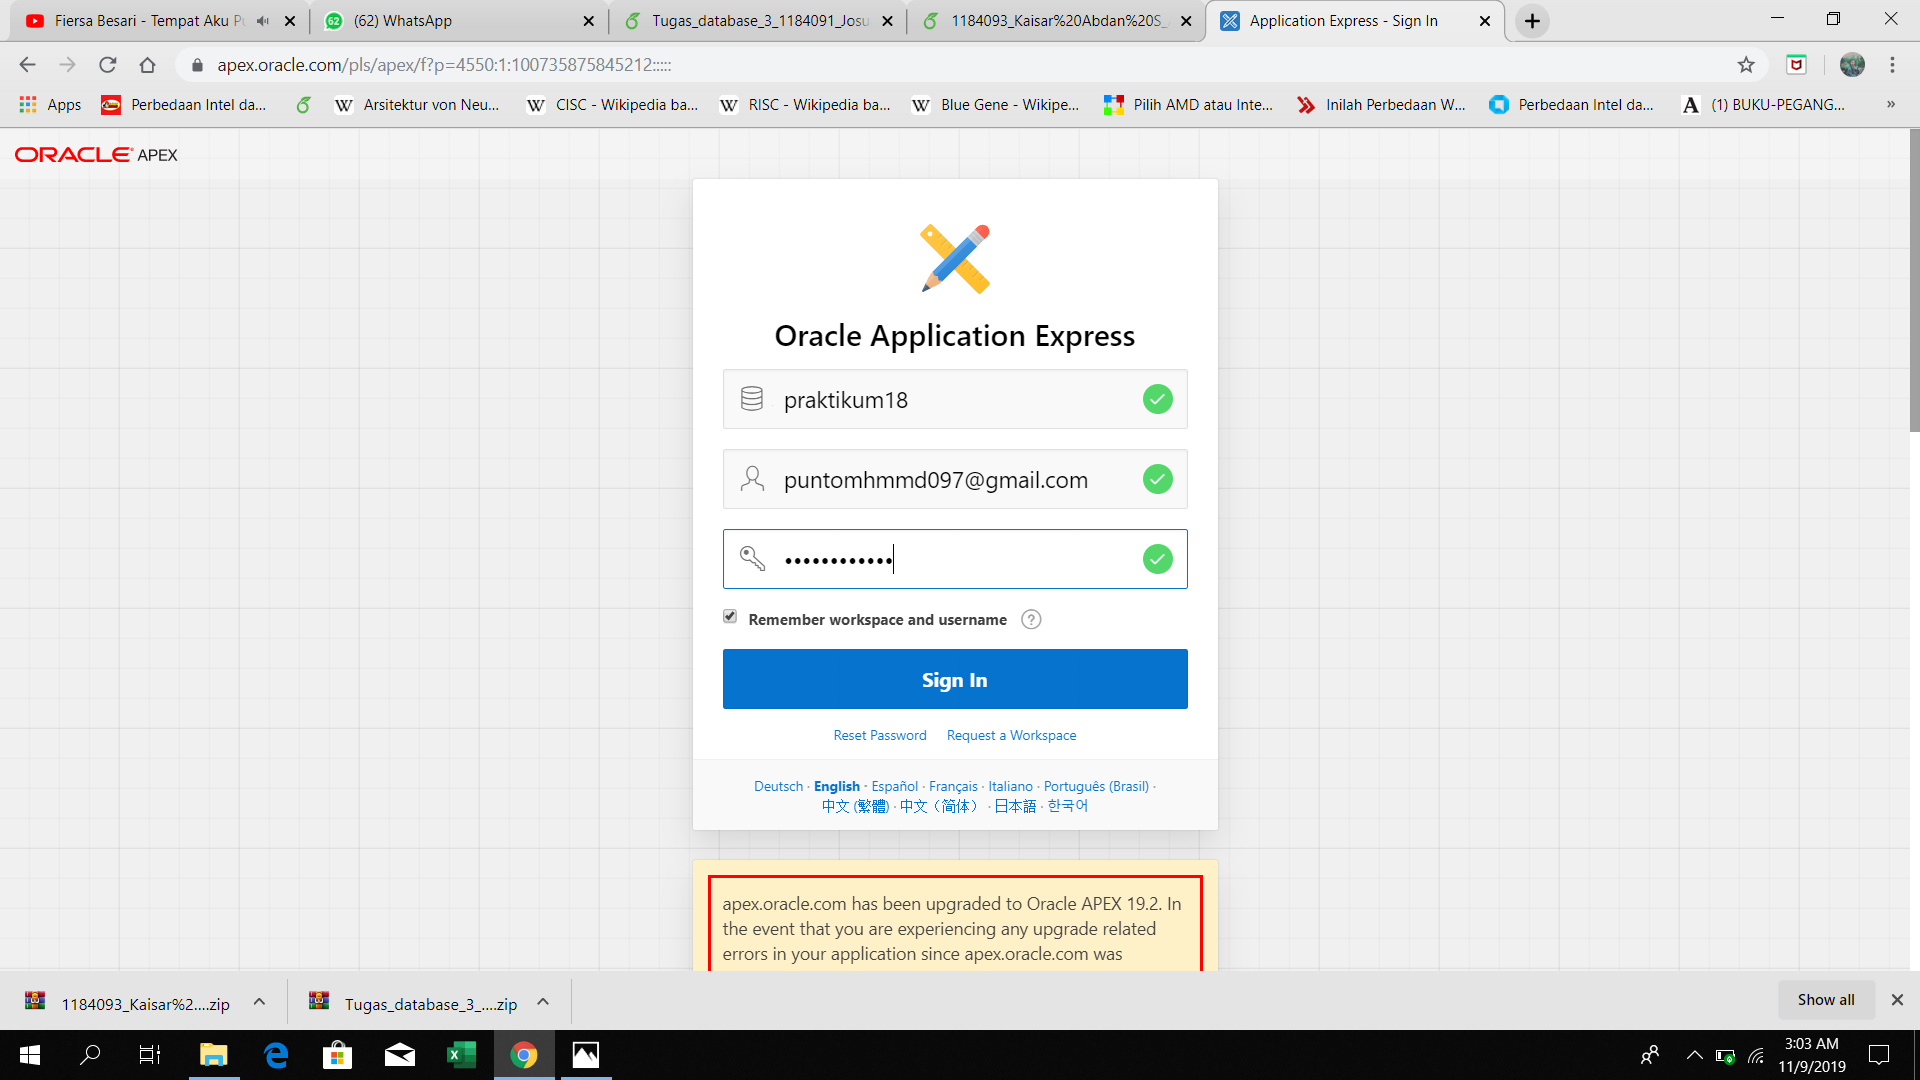
\includegraphics[scale=0.2]{figures/29.png}
     \caption{Login Apex Online}
    \end{center}   
    \end{figure}

\begin{figure}[!htbp]
\item[3]Setelah masuk ke akun oracle apex online dan workspace masing-masing, kemudian klik App Builder dan pilih create.

    \begin{center}
    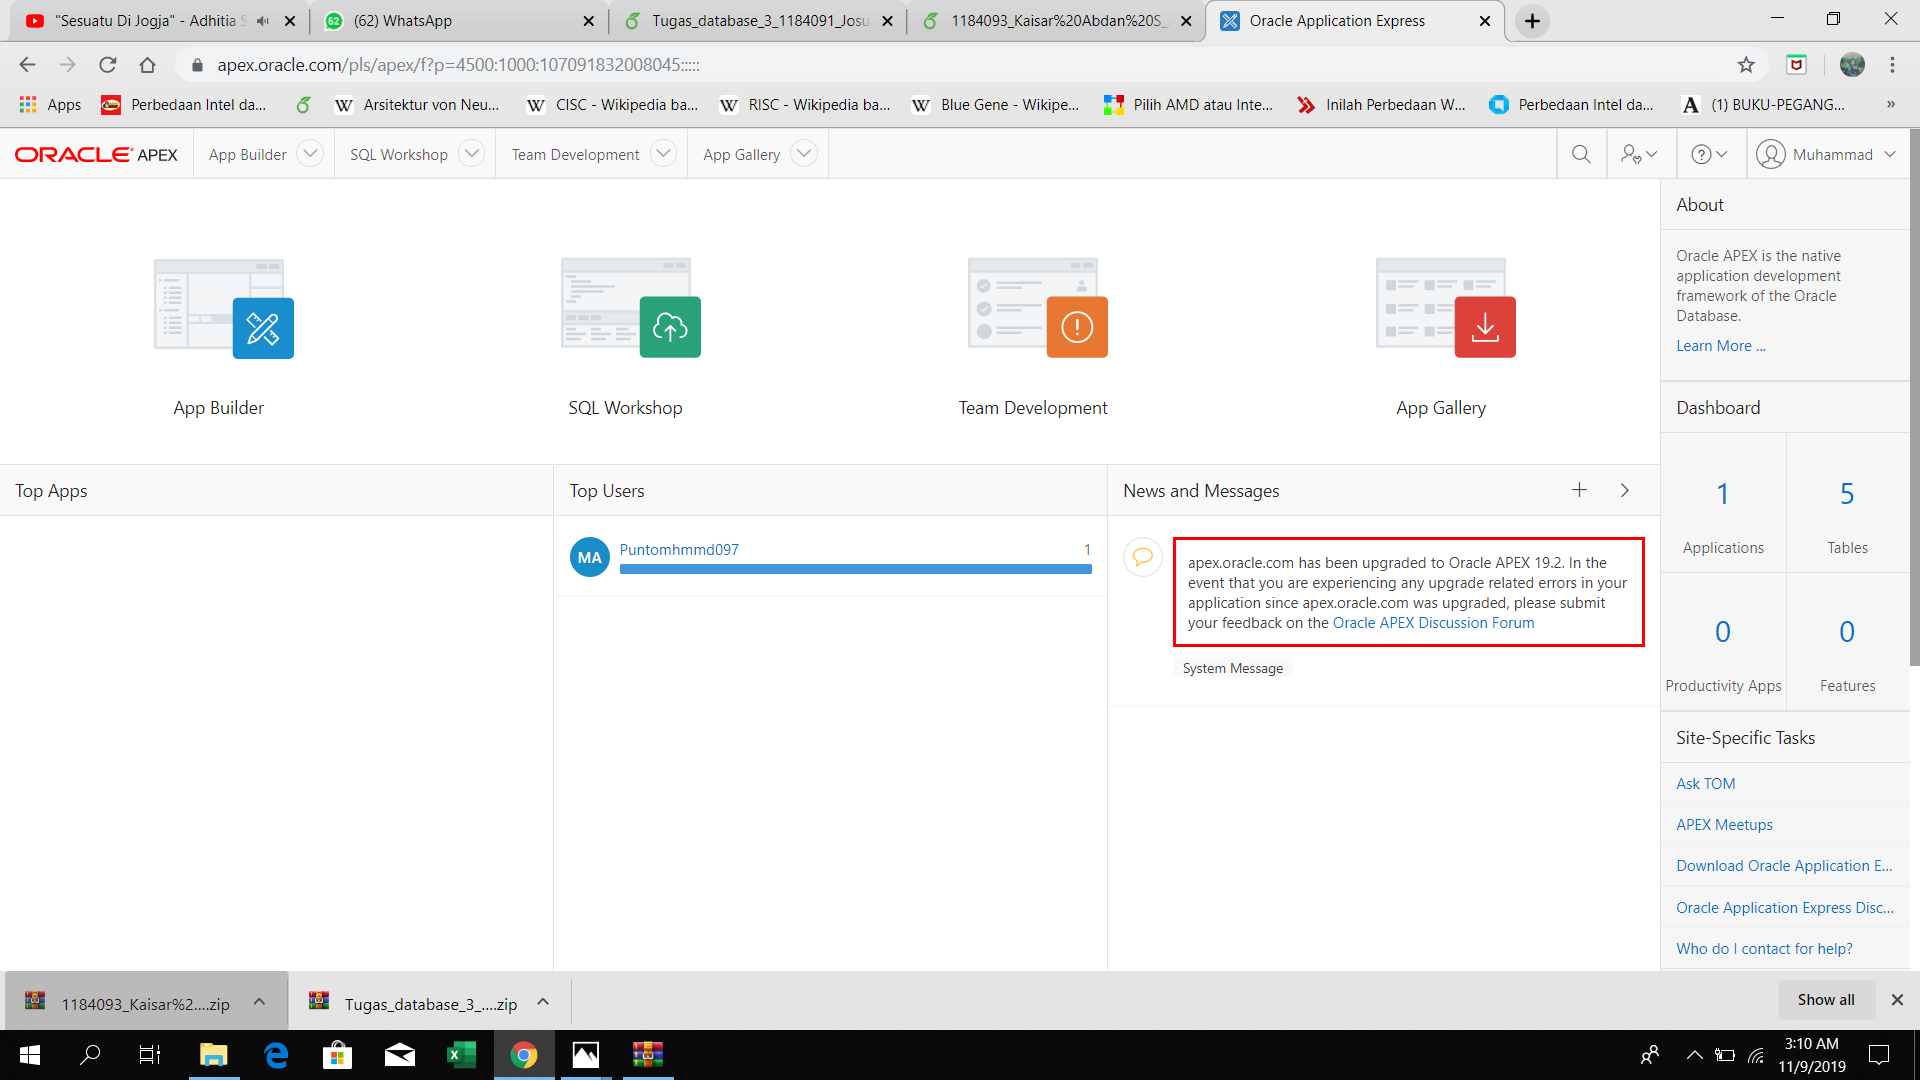
\includegraphics[scale=0.2]{figures/30.png}
     \caption{Tampilan Utama Apex Online}
    \end{center}   
    \end{figure}

\begin{figure}[!htbp]
\item[4]Kemudian Pilih 'from a file'. Di menu ini kita mengupload data/project kita yang telah dibuat pada Microsoft Excel untuk dijadikan sebuah aplikasi.


    \begin{center}
    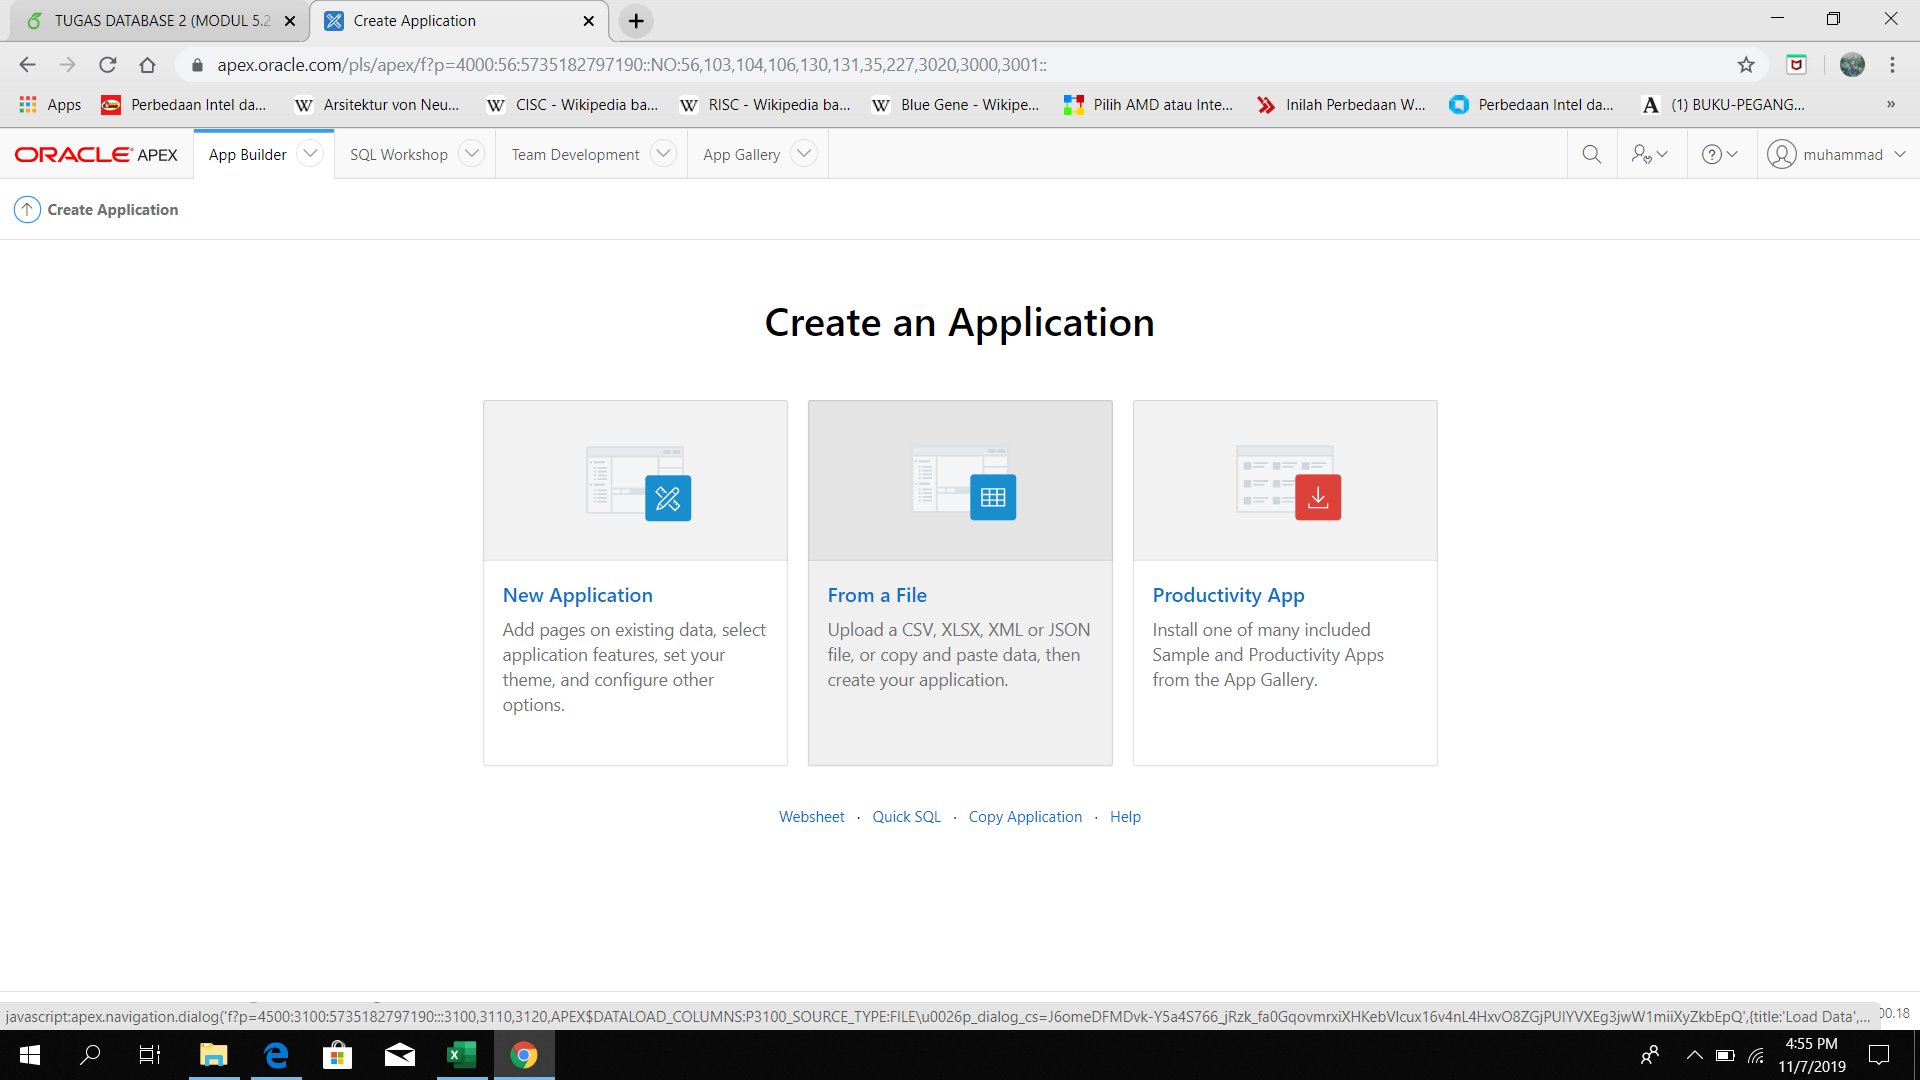
\includegraphics[scale=0.2]{figures/7.png}
     \caption{Tampilan Form Create Aplication}
    \end{center}   
    \end{figure}

\newpage
\item[5]Kemudian pilih file excel yang telah disimpan untuk diupload.

\begin{figure}[!htbp]
    \begin{center}
    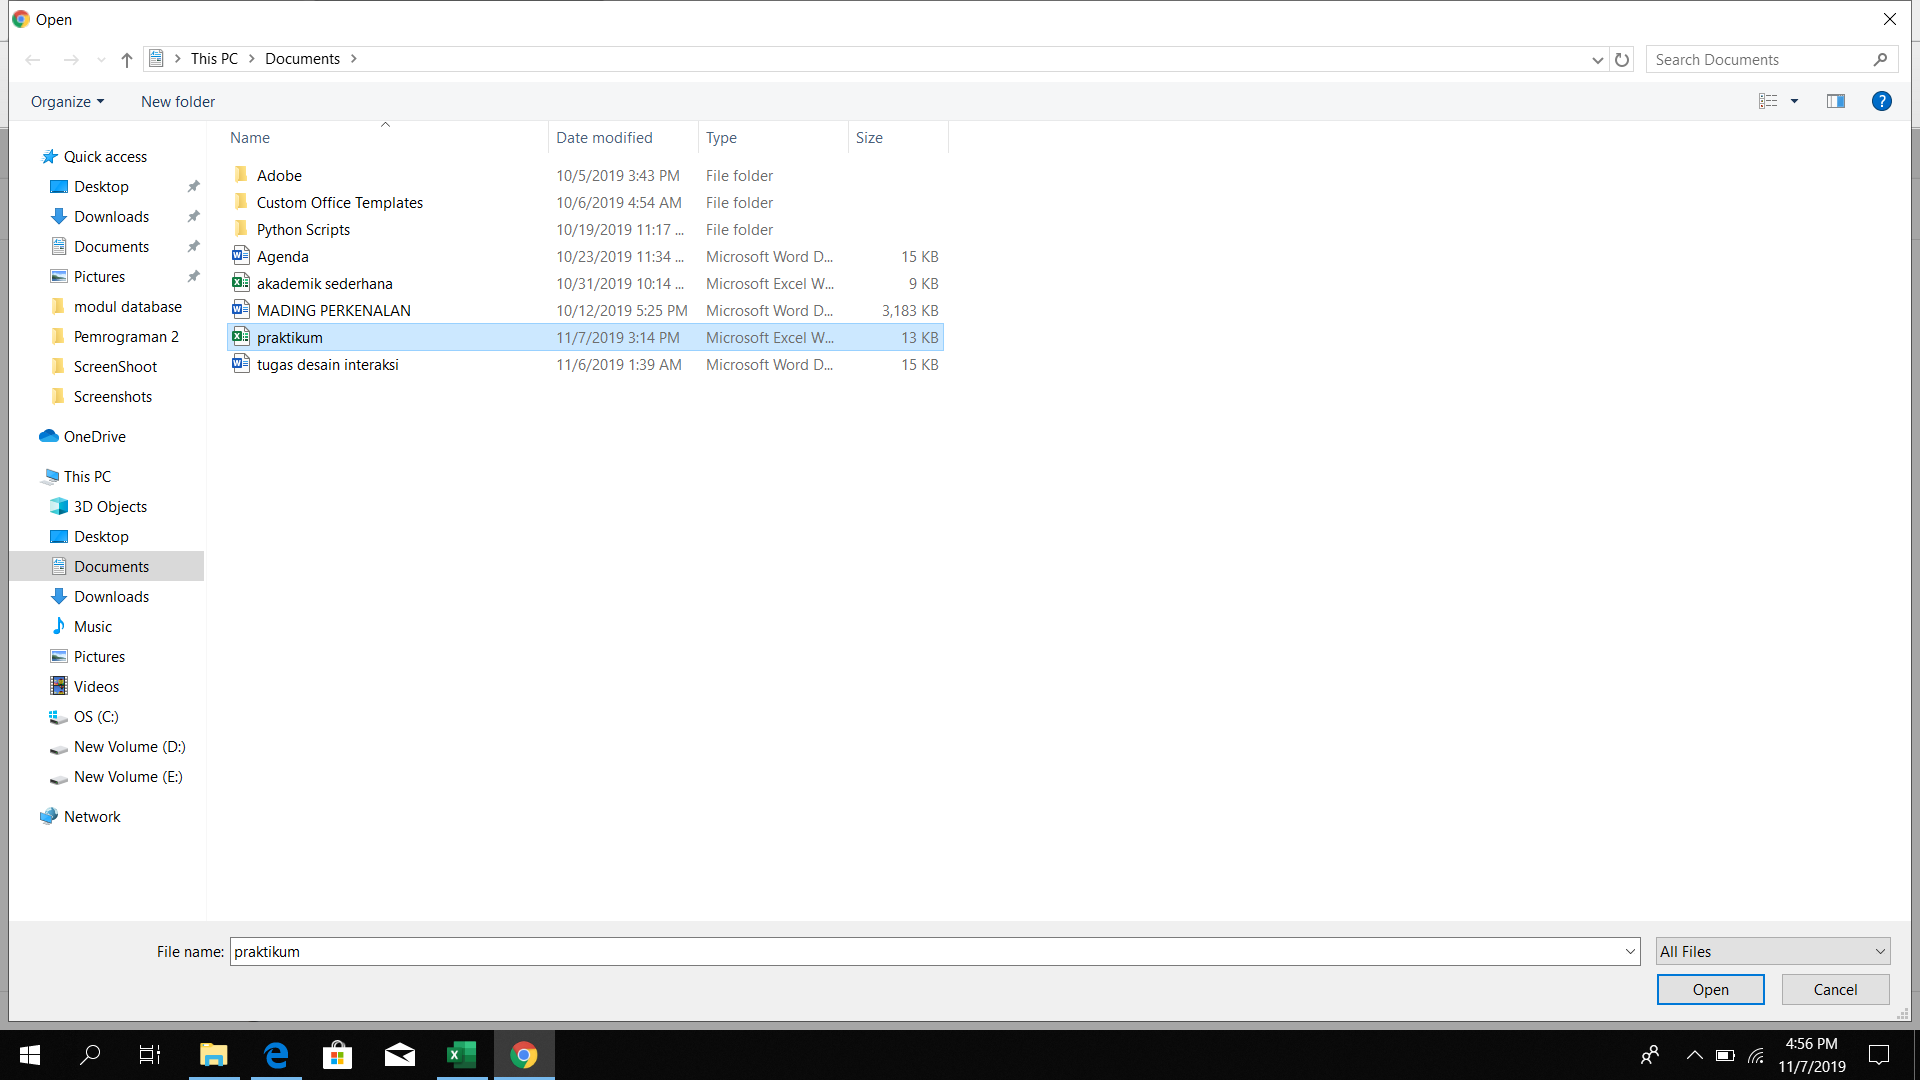
\includegraphics[scale=0.2]{figures/8.png}
     \caption{Pilih file Excel}
    \end{center}   
    \end{figure}

\item[6]Selanjutnya kita masuk pada form load data. Disini kita melakukan input nama pada kolom table name. setelah memasukkan inputan nama pada kolom table name, kita memilih sheet/tabel yang telah dibuat sesuai dengam nama tabel yang dibuat. Misal, ketika menginputkan 'mahasiswa' pada table name maka sheet/tabel yang dipilih adalah tabel mahasiswa. Begitupun untuk empat tabel selanjutnya, yaitu dosen, kuliah, jadwal,dan nilai.

\begin{figure}[!htbp]
    \begin{center}
    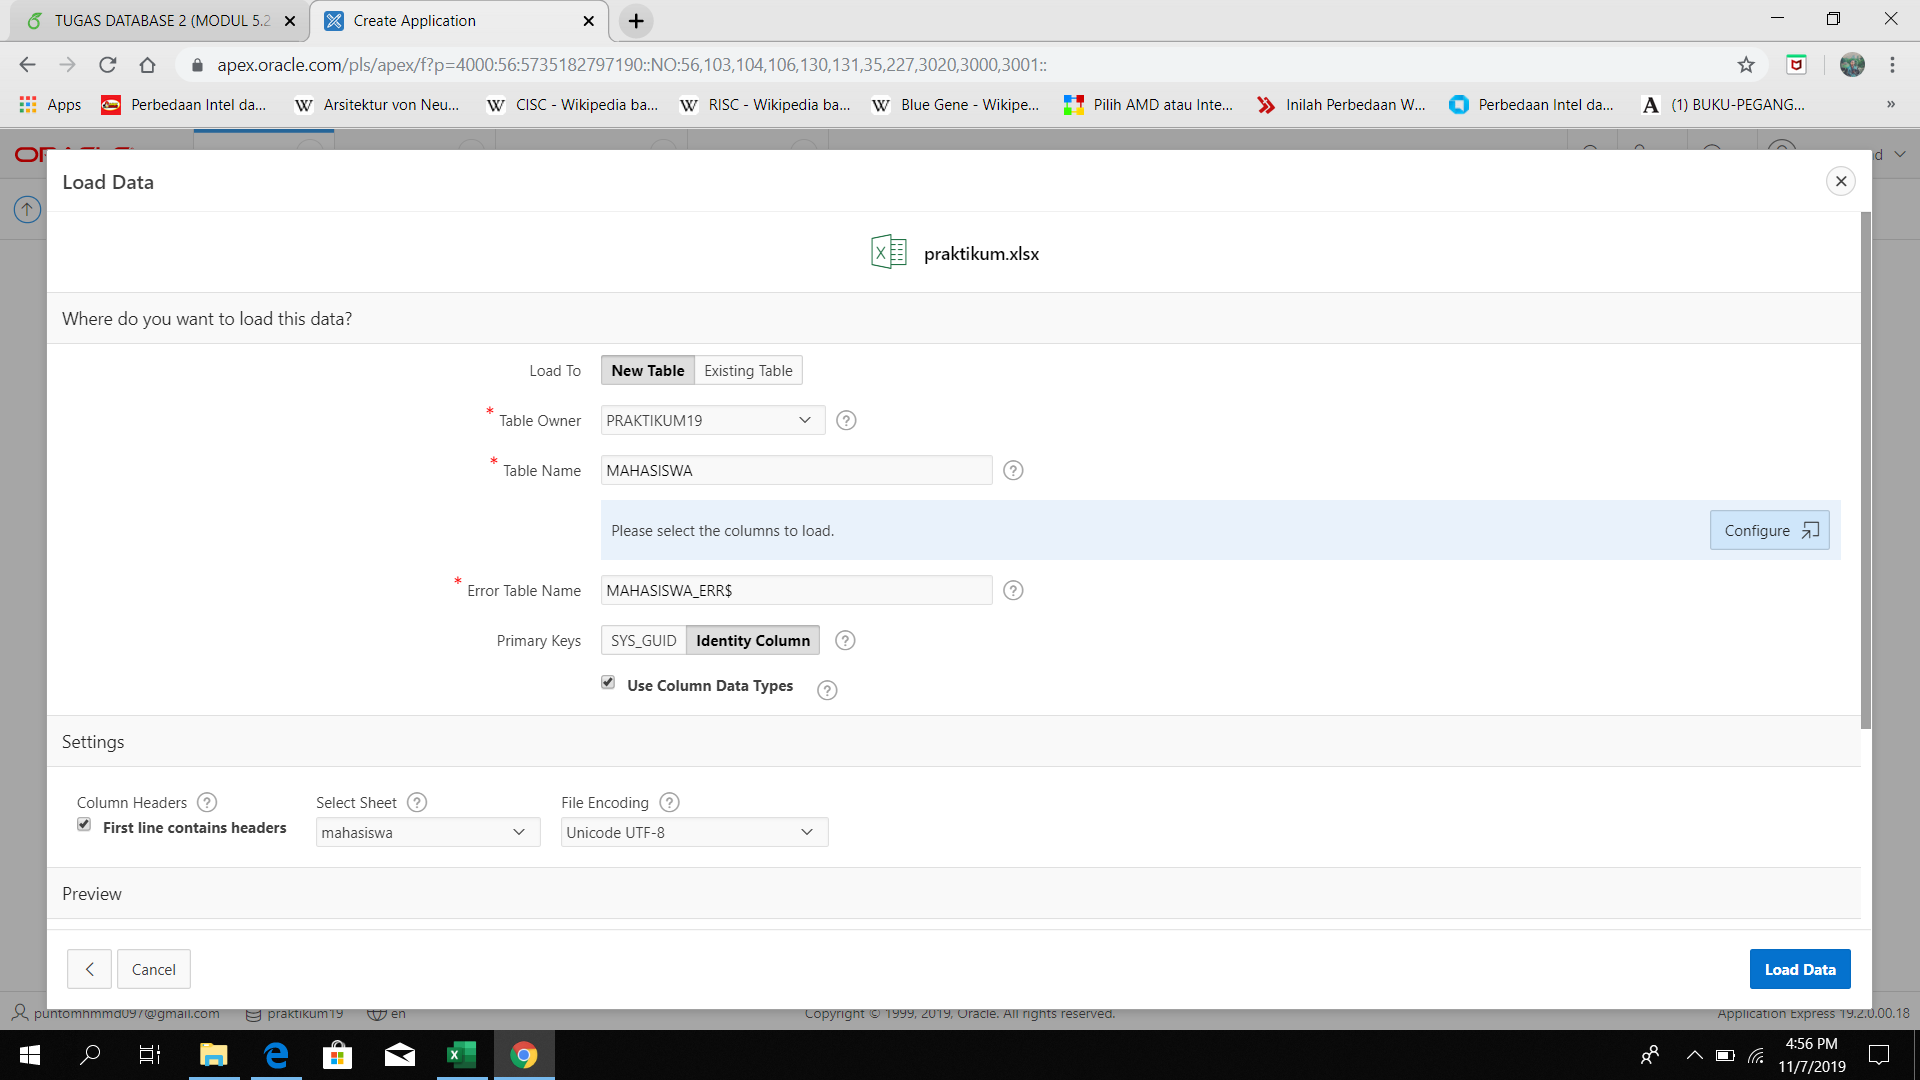
\includegraphics[scale=0.2]{figures/9.png}
     \caption{Tampilan form load data}
    \end{center}   
    \end{figure}
    
\begin{figure}[!htbp]
\item[7]Setelah kelima tabel (mahasiswa, dosen, kuliah, jadwal, dan nilai) telah terbuat, kemudian pilih SQL Workshop.

    \begin{center}
    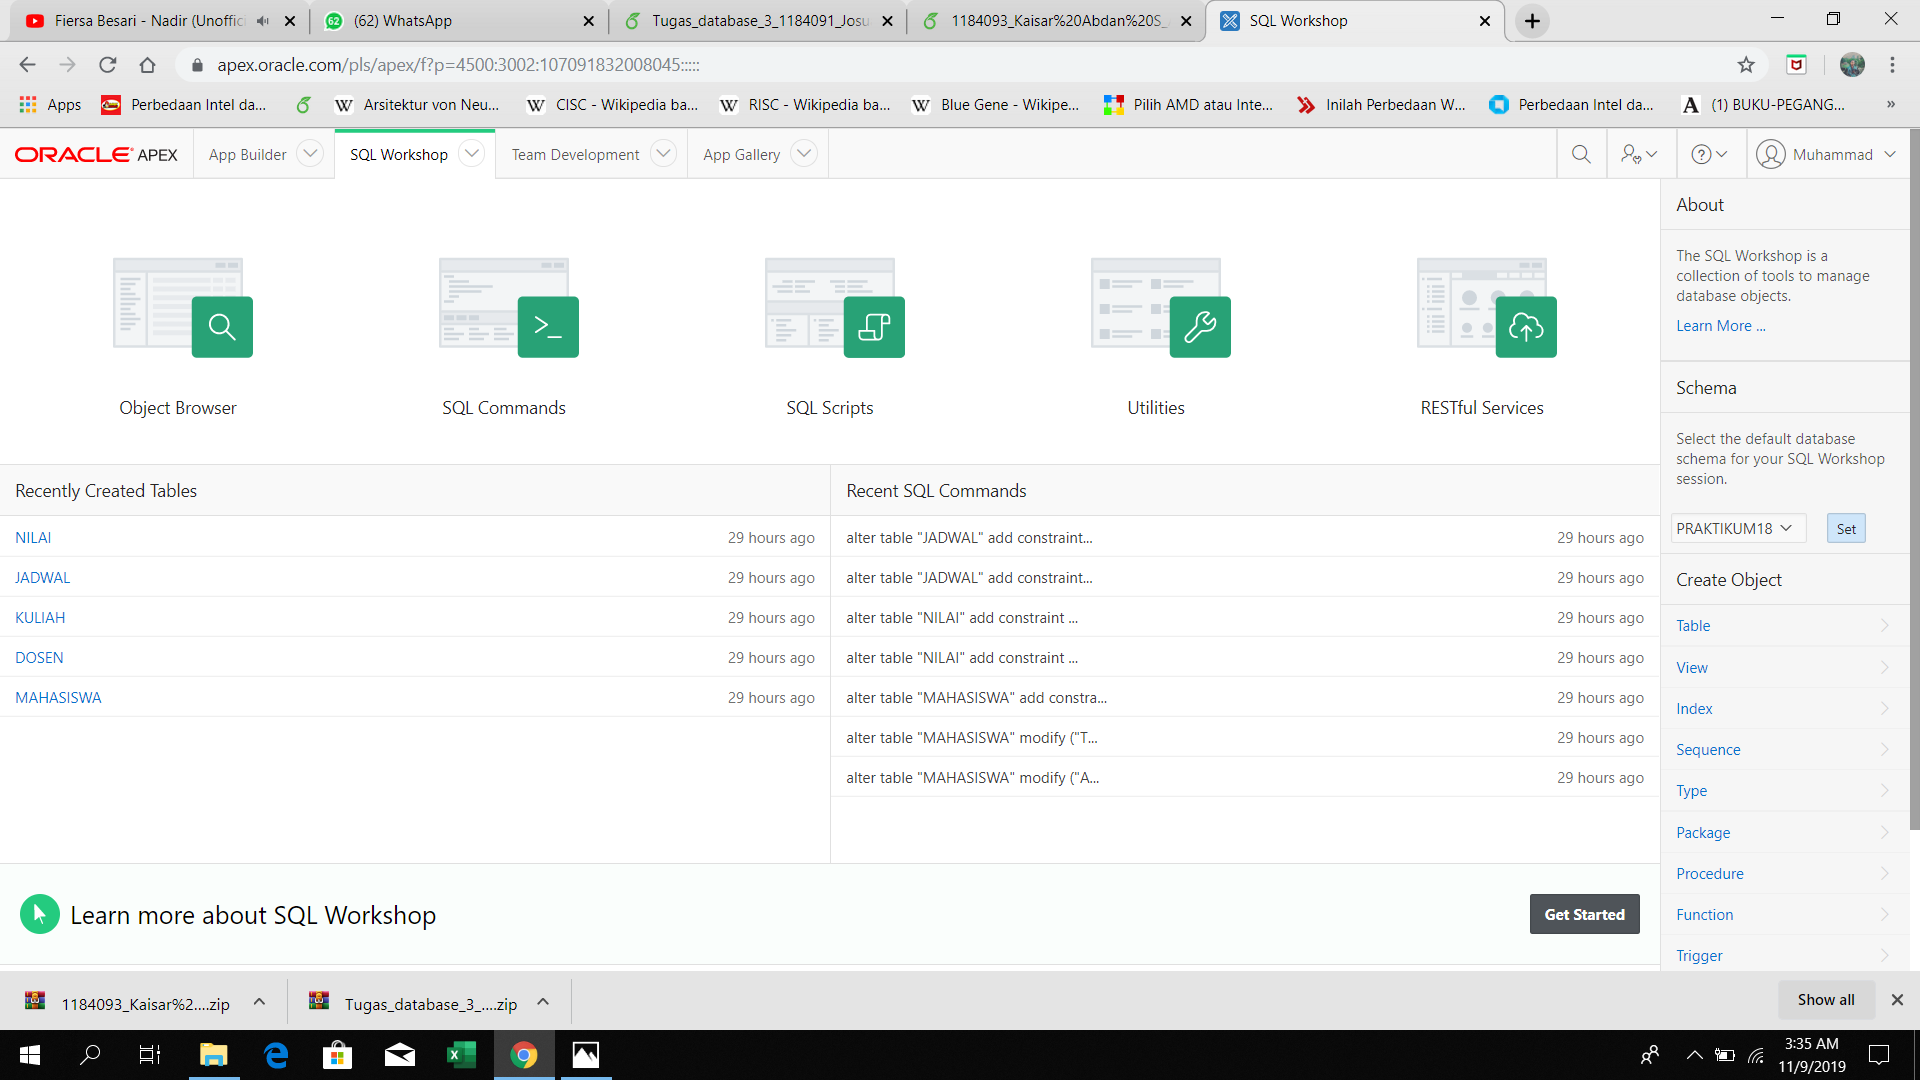
\includegraphics[scale=0.2]{figures/31.png}
     \caption{Tampilan halaman SQL Workshop}
    \end{center}   
    \end{figure}
    
\begin{figure}[!htbp]
\item[8]setelah itu dapat dilakukann pengecekan pada setiap tabel yang telah terbuat. Ketika melakukan pengecekan, setiap tabel yang telah dibuat mendapat tambahan kolom ID sebagai primary key untuk setiap tabel. Hal ini terjadi karena sebelumnya untuk setiap tabel yang dibuat belum mempunyai primary key. Untuk menghapus kolom ID ini dapat dengan memilih pilihan Drop Colmun.

    \begin{center}
    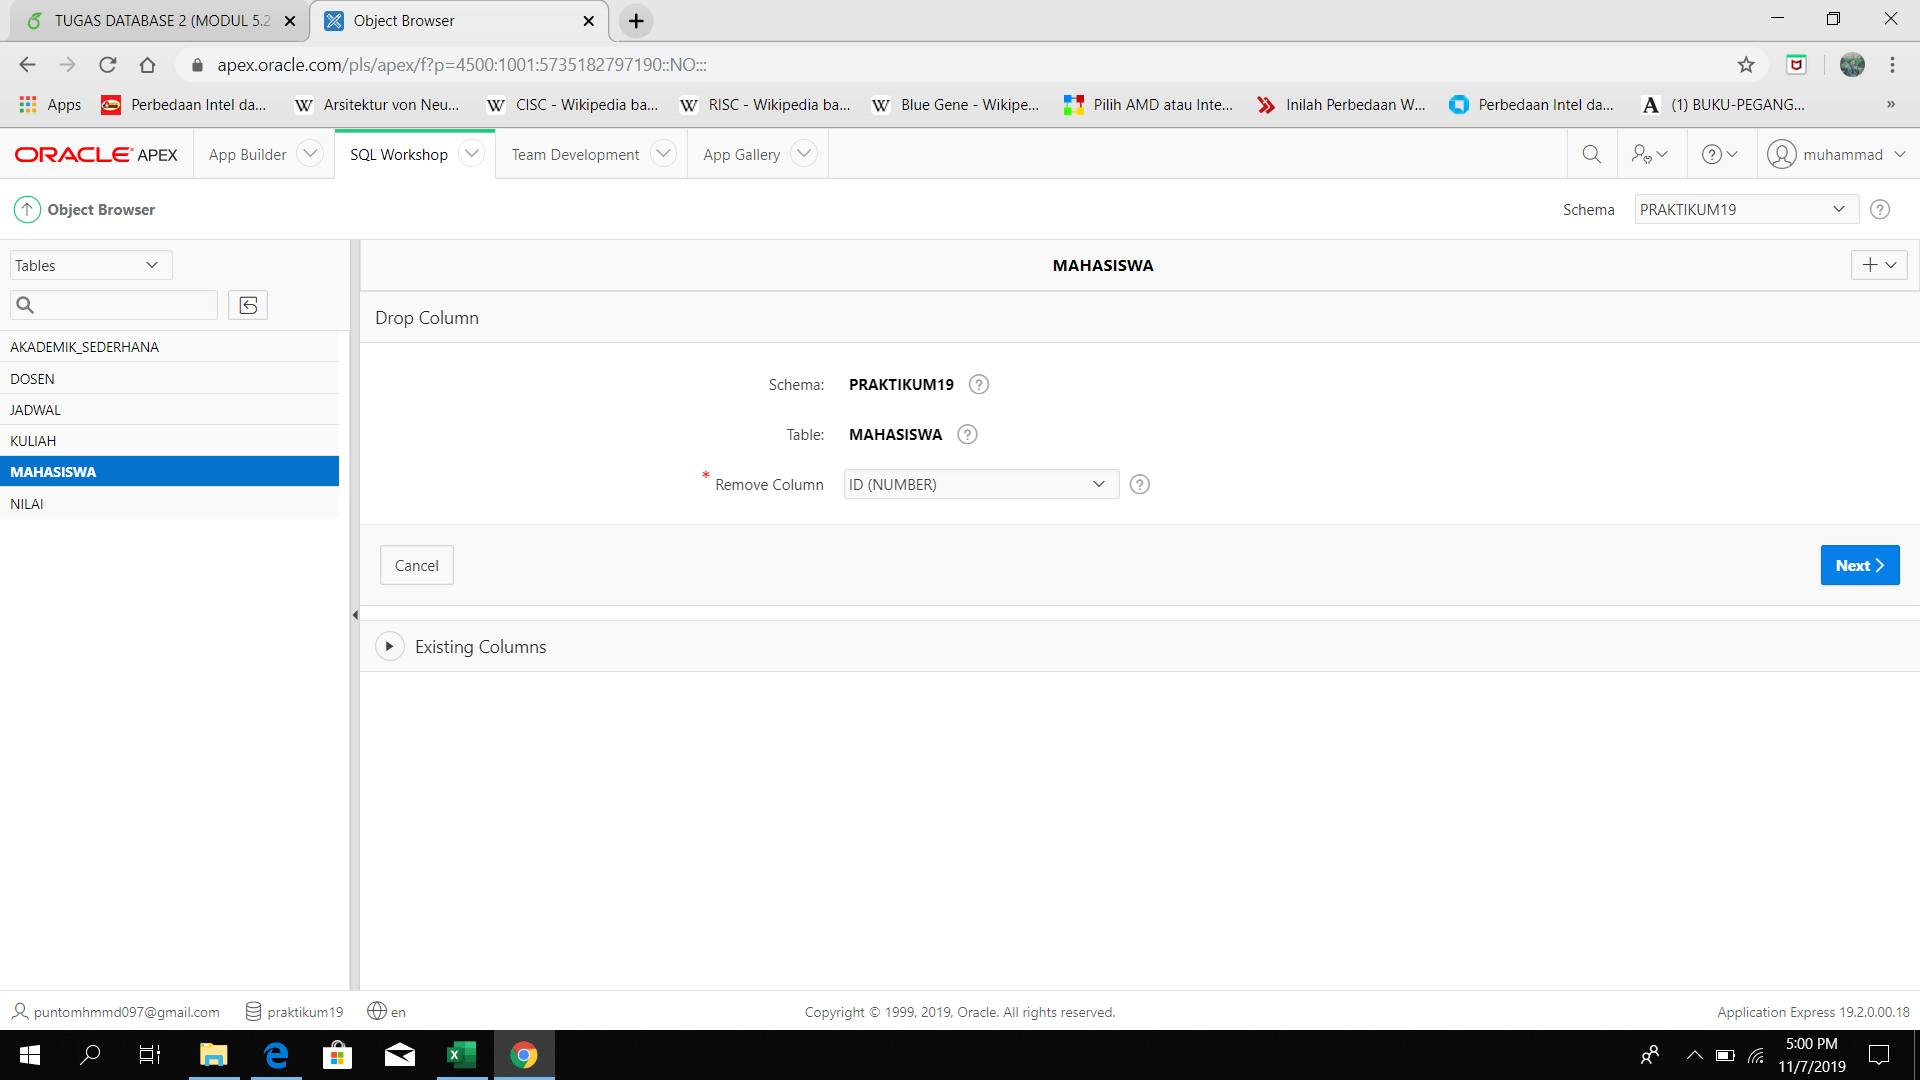
\includegraphics[scale=0.2]{figures/15.png}
     \caption{Tampilan halaman object browser}
    \end{center}   
    \end{figure}
    
\begin{figure}[!htbp]   
\item[9]setelah kolom ID pada semua tabel telah terhapus, selanjutnya kita melakukan penentuan prymary key pada tabel. Untuk tabel Mahasiswa primary key yaitu NIM. Untuk tabel Dosen primary key yaitu NIK. Untuk tabel Kuliah primary key yaitu Kode. sedangkan untuk tabel jadwal mempunyai 2 foreign key yaitu KODE dan NIK. Begitupun pada tabel nilai mempunyai 2 foreign key yaitu NIM dan KODE.


    \begin{center}
    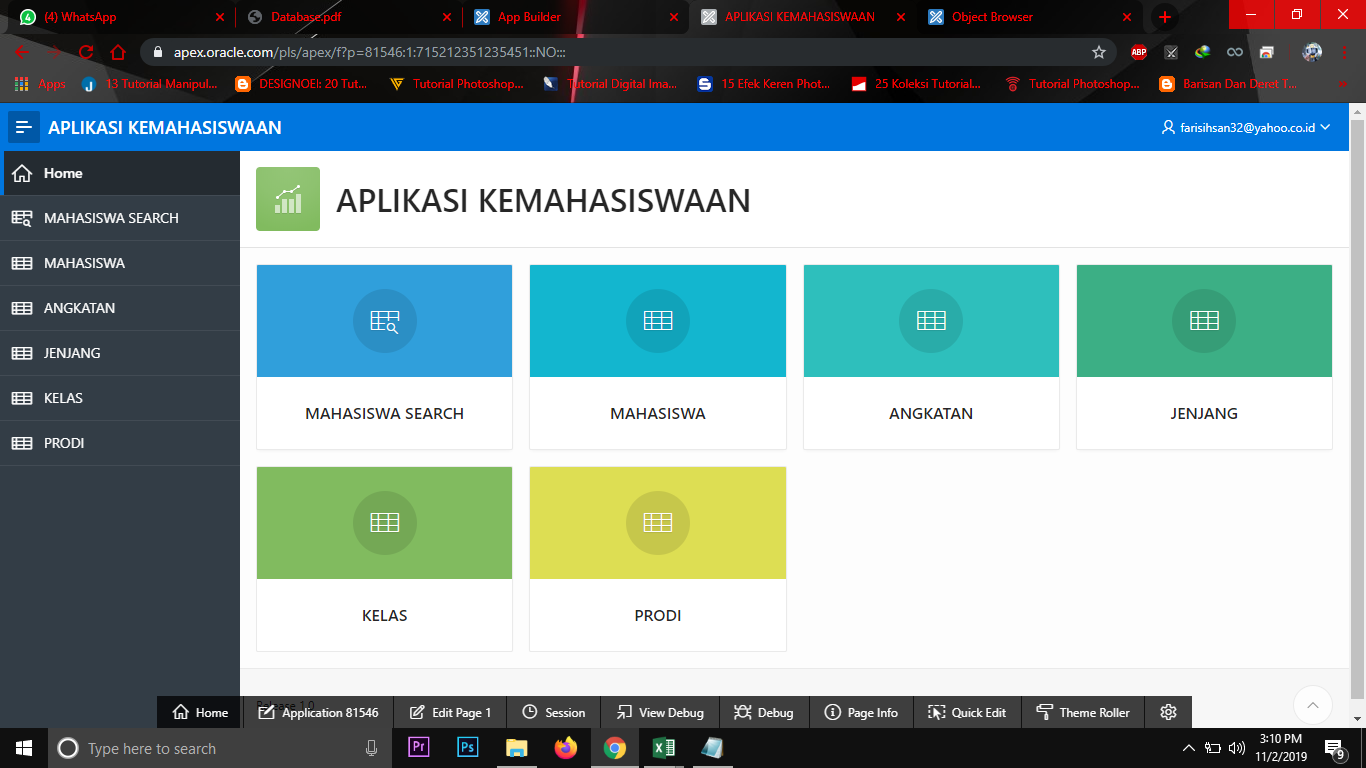
\includegraphics[scale=0.2]{figures/12.png}
     \caption{Tampilan Membuat primary key dan foreign key}
    \end{center}   
    \end{figure}

\begin{figure}[!htbp]
\item[10]Setelah prumary key dan foreign key telah dibuat selanjutnya kita akan membuat apliaksi. Untuk membuat aplikasi dapat pilih APP Builder, kemudian pilih Create dan pilih New Aplication. Selanjutnya masukkan nama aplikasi yang kan dibuat.


    \begin{center}
    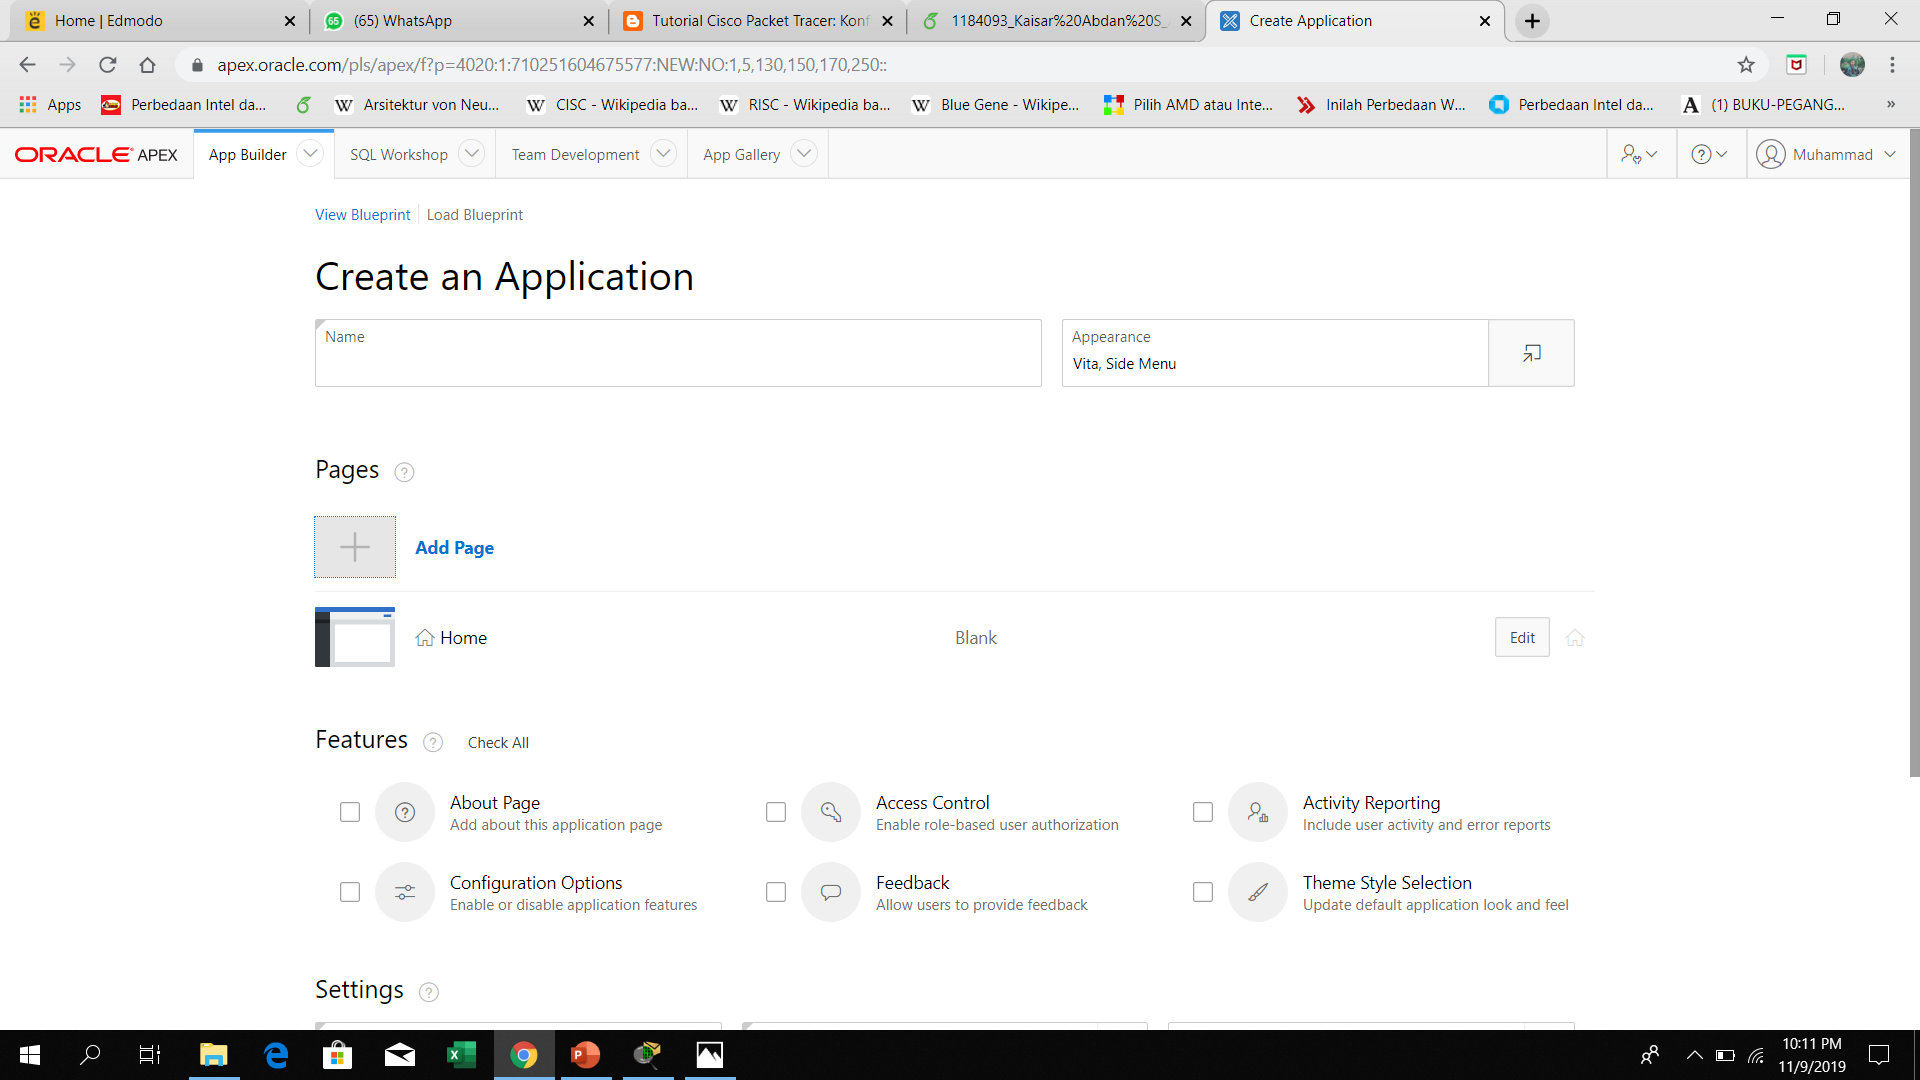
\includegraphics[scale=0.2]{figures/32.png}
     \caption{Tampilan Create Application}
    \end{center}   
    \end{figure}

\begin{figure}[!htbp]
\item[11]Selanjutnya pilih add page. kemudian kita memilih tampilan page. Disini kita memilih tipe Interactive Report. setelah itu kita memasukkan nama page yang akan dibuat.Kemudian kita memilih tabel yang akan dimasukkan. Untuk nama page disesuaikan dengan tabel. Misal tabel yang akan dimasukkan adalah tabel mahasiswa maka untuk nama page yang dibuat adalah mahasiswa. Begitupun untuk tabel dosen, kuliah, jadwal, dan nilai.

    \begin{center}
    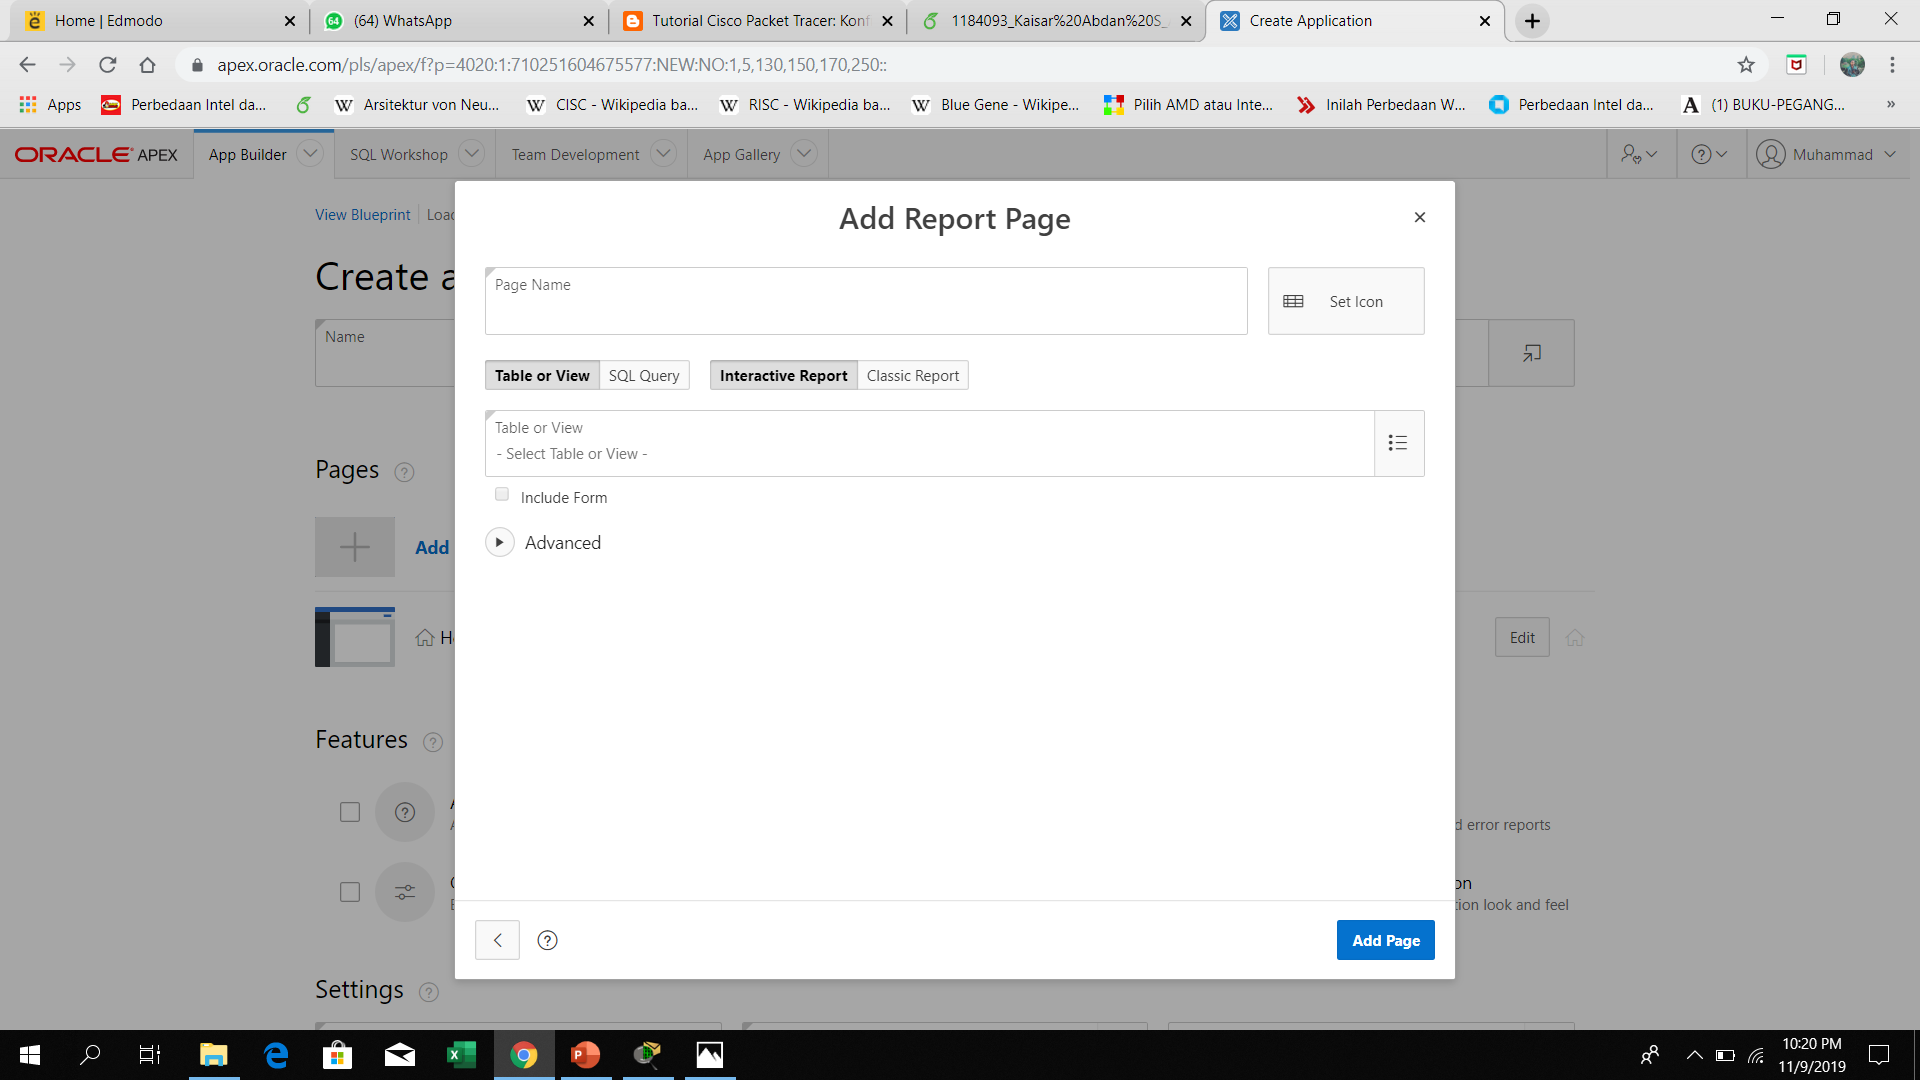
\includegraphics[scale=0.2]{figures/33.png}
     \caption{Tampilan halaman Add Report Page}
    \end{center}   
    \end{figure}
    
\begin{figure}[!htbp]
\item[12]Setelah itu dapat juga ditambahkan page dashbord pada aplikasi yang akan dibuat. Page dashbord ini berisi tentang grafik. 

    \begin{center}
    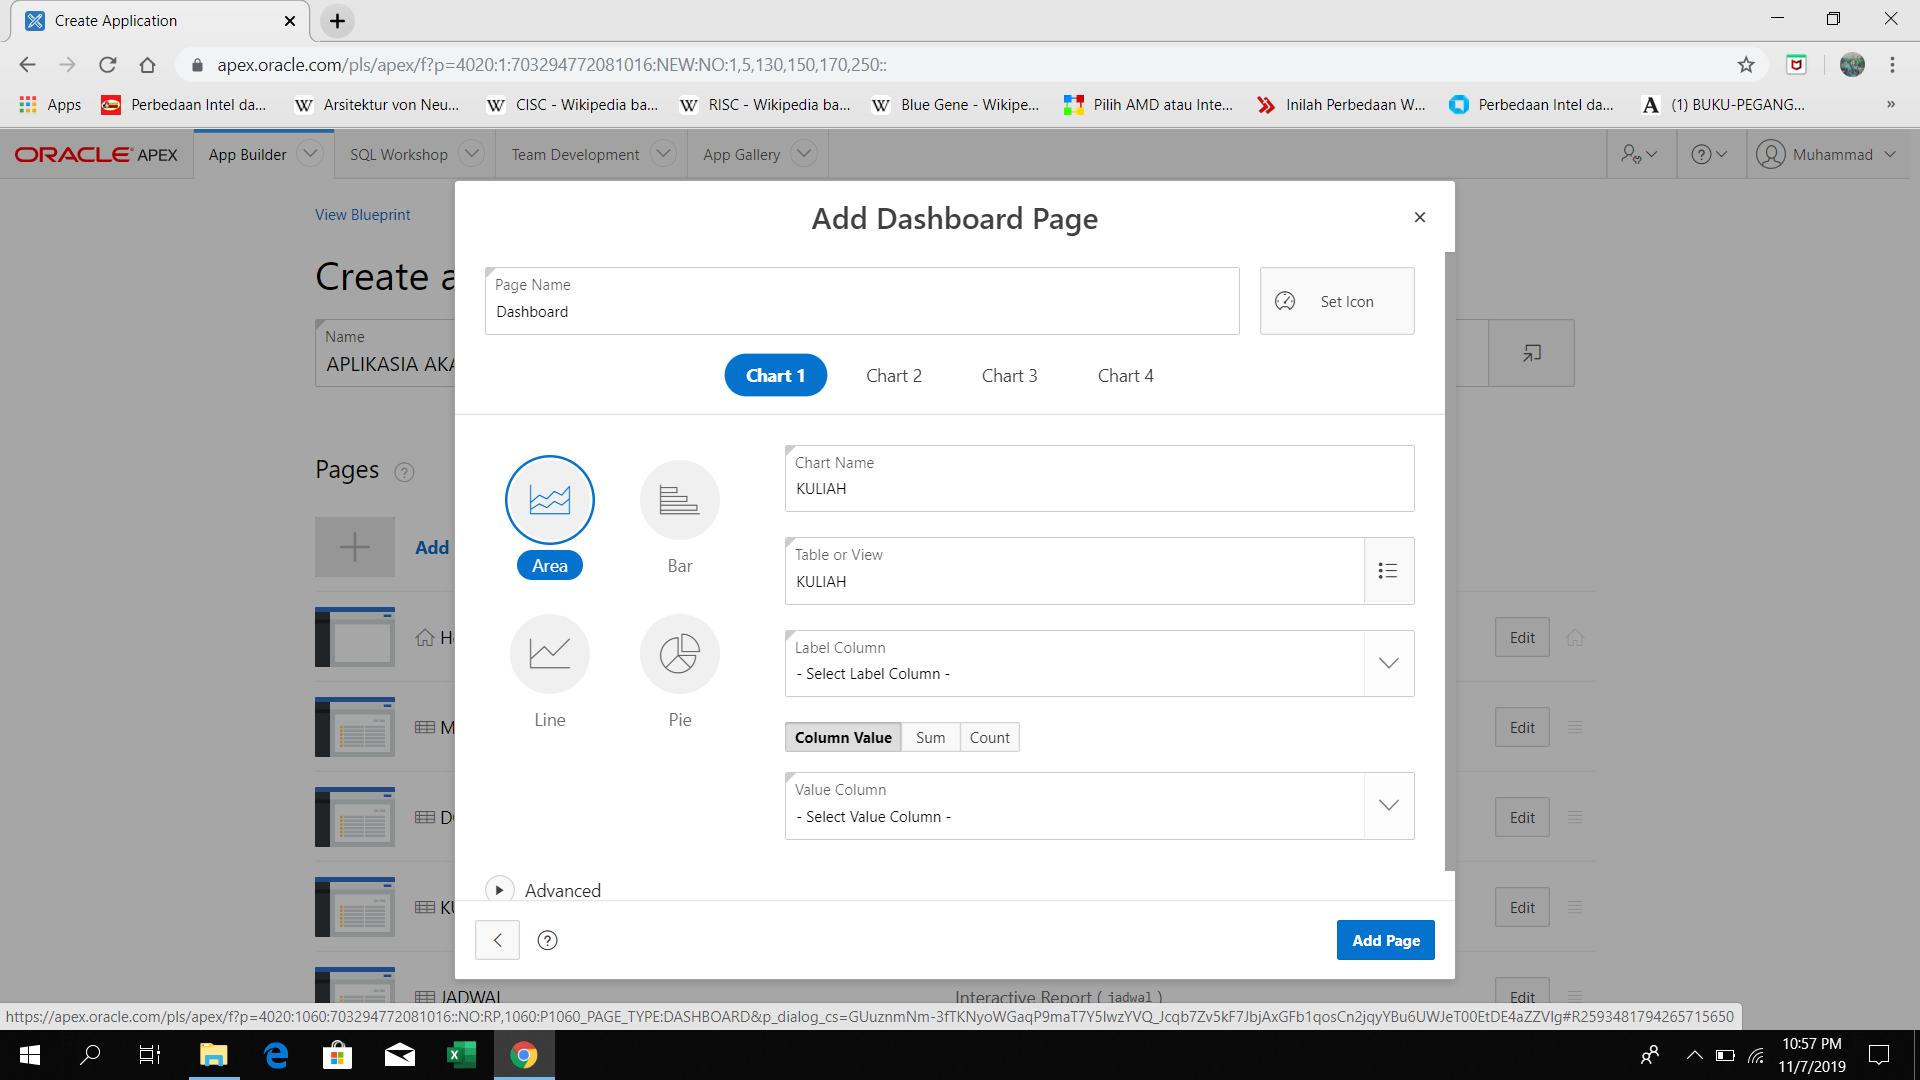
\includegraphics[scale=0.2]{figures/25.png}
     \caption{Tampilan halaman Add Dashbord Page}
    \end{center}   
    \end{figure}
 
\begin{figure}[!htbp]   
\item[13]setelah semua page telah terbuat, kemudian klik finish. setelah itu kita run aplication. Pada Run Application kita masukkan username dan password.\\
Aplikasi : https://apex.oracle.com/pls/apex/f?p=93947:1:706169586111906:::::\\
username : puntomhmmd097@gmail.com\\
password : bismillah721


    \begin{center}
    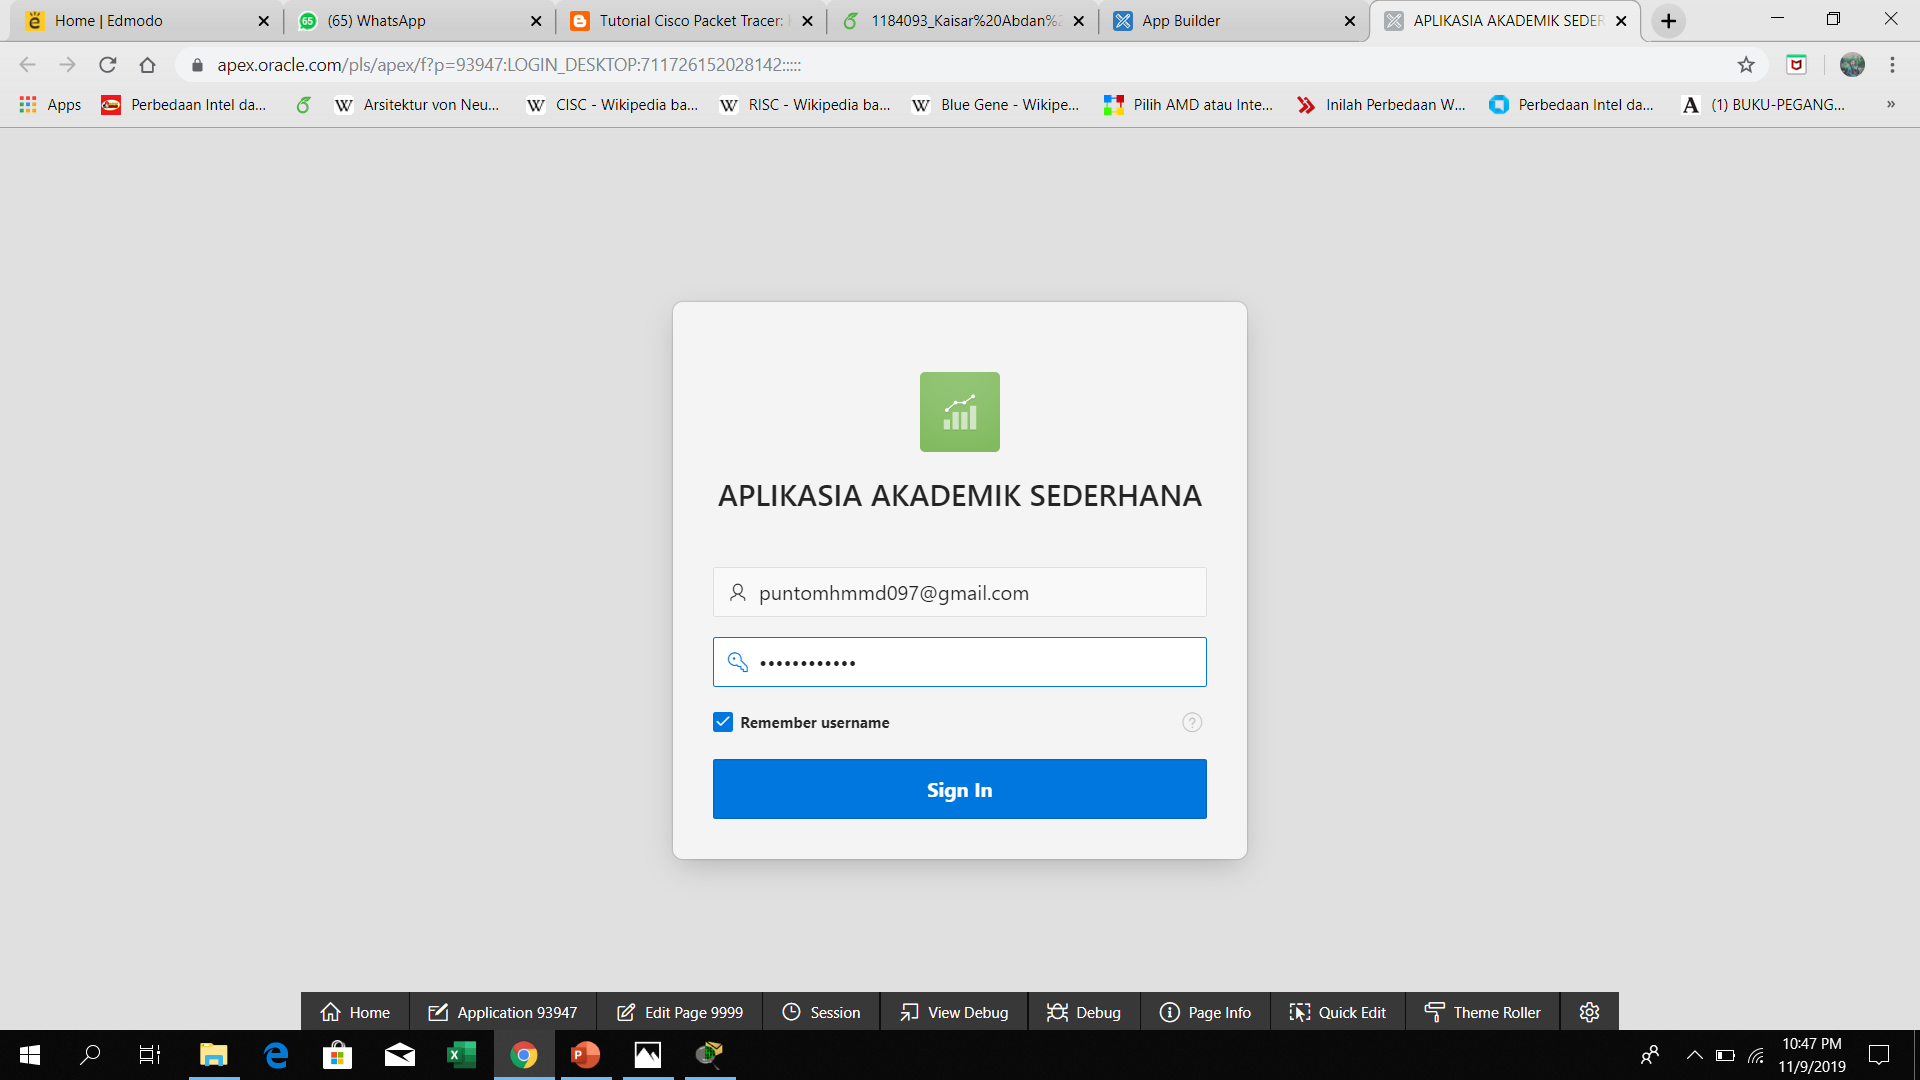
\includegraphics[scale=0.2]{figures/34.png}
     \caption{Tampilan login ke Aplikasi}
    \end{center}   
    \end{figure}

\begin{figure}[!htbp]
\item[14]Setelah menginputkan username dan password anda akan masuk ke dalam aplikasi.Berikut adalah tampilan aplikasi.

    \begin{center}
    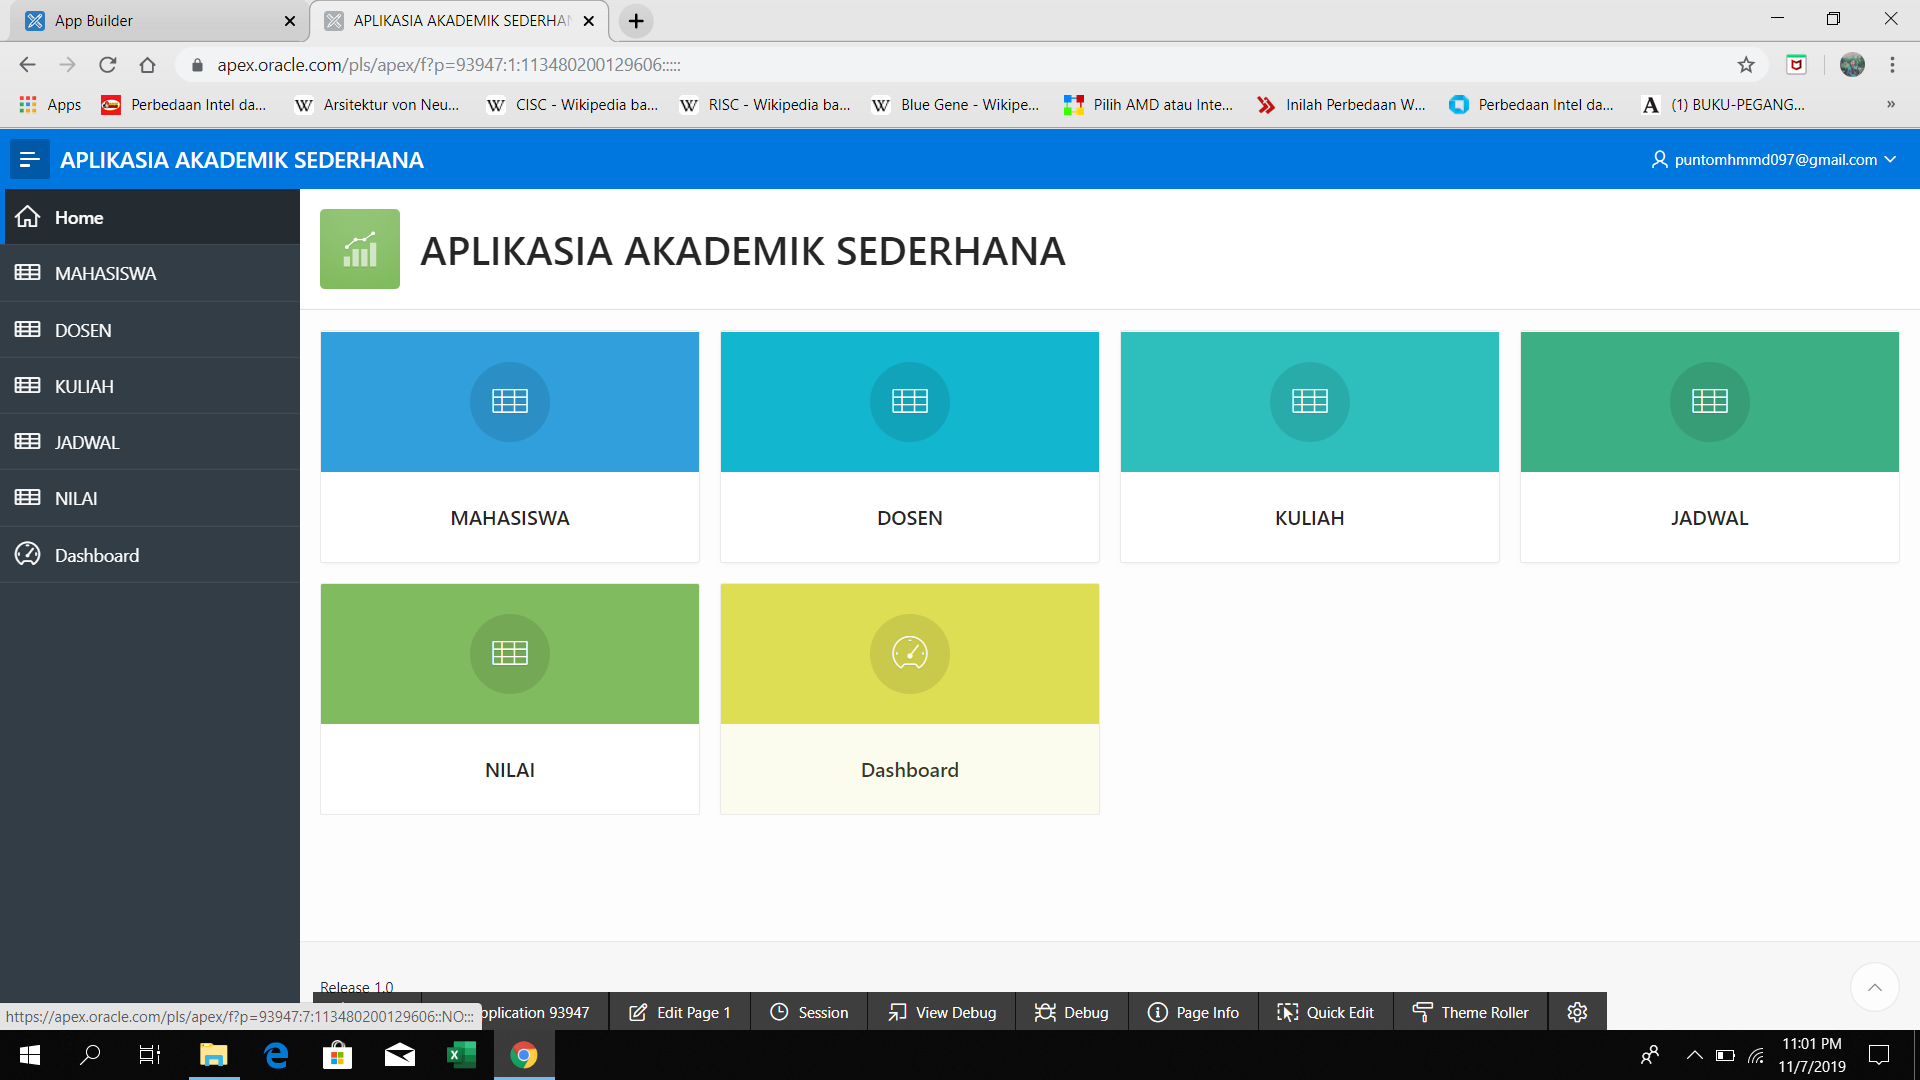
\includegraphics[scale=0.2]{figures/28.png}
     \caption{Tampilan Aplikasi yang dibuat}
    \end{center}   
    \end{figure}

\end{enumerate}


